% Module 7: Multi-Agent Systems - Short Assignment
% Compile with XeLaTeX: latexmk -xelatex -interaction=nonstopmode report.tex
\documentclass{article}

\PassOptionsToPackage{numbers,compress}{natbib}
\usepackage[final]{template22}
% Layout for the Module 7 PPO short report.
\usepackage[T1]{fontenc}
\usepackage{microtype}
\usepackage{times}
\usepackage{graphicx}
\usepackage{amsmath,amssymb}
\usepackage{enumitem}
\usepackage{booktabs,tabularx,array}
\usepackage[skip=3pt,font=small]{caption}
\usepackage[pagebackref=true,breaklinks=true,colorlinks]{hyperref}
\usepackage{xspace}

\hypersetup{
  pdfencoding=auto,
  colorlinks=true,
  allcolors=black
}

\usepackage{fancyhdr}
\renewcommand{\headrulewidth}{0.5pt}
\renewcommand{\footrulewidth}{0pt}
\fancyhf{}
\fancyfoot[C]{\thepage}

\setlength{\floatsep}{0.5\baselineskip plus 3pt minus 2pt}
\setlength{\textfloatsep}{0.5\baselineskip plus 3pt minus 2pt}
\graphicspath{{figures/}}


\title{Proximal Policy Optimization on CartPole}

\author{%
  Yuanze Lei \quad 2510124204\\
  Peking University
}

\begin{document}
\maketitle

\begin{abstract}
This short study implements proximal policy optimization (PPO) for the
discrete CartPole control task. The actor samples actions from a softmax
policy; the critic estimates state value with a one-step temporal-difference
target; and generalized advantage estimation supplies the relative signal used
by the clipped policy objective. In one fixed-seed run of 500 episodes, the
mean return rises from 140.26 in the first 100 episodes to 199.19 in the last
100. The final 100 episodes reach the 200-step evaluation limit 96 times and
never fall below 173. These results support stable control within the
environment's evaluation window, not an empirical proof of indefinitely long
balance.
\end{abstract}

\section{Task and Learning Signal}\label{sec:task}

CartPole \citep{brockman2016gym} is an underactuated balance problem. At each
step, the agent observes position, cart velocity, pole angle, and angular
velocity. It applies one of two fixed horizontal forces, left or right. It
receives reward one while the pole remains within its angular limit and the
cart remains within the track. An episode ends on either failure or the 200
step time limit.

Because the environment observes only 200 steps, a return of 200 means that
the policy survived the evaluation window. The underlying dynamical system
does not acquire a proof of perpetual balance from that observation. We
therefore distinguish finite-horizon control performance from long-term
stability when interpreting the measured curve.

The actor outputs a probability for each discrete action and samples the
executed action from that distribution. For the trajectory
$(s_t,a_t,r_t,s_{t+1},d_t)$, the critic estimates $V_\theta(s_t)$ and the
one-step target is
\begin{equation}\label{eq:td}
  y_t=r_t+\gamma V_\theta(s_{t+1})(1-d_t),
\end{equation}
with $\gamma=0.98$. Its temporal-difference error is
\begin{equation}\label{eq:delta}
  \delta_t=y_t-V_\theta(s_t).
\end{equation}
Generalized advantage estimation \citep{schulman2015high} accumulates
these errors backwards with $\lambda=0.95$:
\begin{equation}\label{eq:gae}
  \hat A_t=\delta_t+\gamma\lambda\hat A_{t+1}.
\end{equation}
Positive $\hat A_t$ increases the preference for the sampled action; negative
values decrease it.

\section{PPO Update}\label{sec:ppo}

The actor probabilities before the update define
$\pi_{\mathrm{old}}(a_t\mid s_t)$. Re-evaluating the actor during the update
gives $\pi_{\theta}(a_t\mid s_t)$ and the probability ratio
\begin{equation}\label{eq:ratio}
  \rho_t=
  \frac{\pi_{\theta}(a_t\mid s_t)}
       {\pi_{\mathrm{old}}(a_t\mid s_t)}.
\end{equation}
The clipped surrogate objective is
\begin{equation}\label{eq:clip}
  L^{\mathrm{CLIP}}(\theta)=
  \mathbb E\left[
  \min\left(\rho_t\hat A_t,
  \operatorname{clip}(\rho_t,1-\epsilon,1+\epsilon)\hat A_t
  \right)\right],
\end{equation}
with $\epsilon=0.2$ \citep{schulman2017proximal}. Training minimizes
$-L^{\mathrm{CLIP}}$. The clipped term limits further reward for moving a
sampled action toward a favorable direction beyond the ratio interval. It
also preserves an unfavorable direction of correction when the advantage is
negative.

The critic minimizes
\begin{equation}\label{eq:critic}
  L_V(\theta)=\frac{1}{|B|}\sum_{t\in B}
  \left(V_\theta(s_t)-y_t\right)^2.
\end{equation}
Targets are detached from the critic graph. Actor and critic have separate
Adam optimizers and are updated for ten passes over each collected episode.
The implementation also fills and checks the supplied
\texttt{ReplayBuffer.sample} interface, including dictionary transitions. The
PPO training loop itself is on-policy: it collects one episode and updates
from that episode immediately without replaying it.

\section{Experimental Setup}\label{sec:setup}

Table~\ref{tab:setup} lists the prescribed settings. A single seed controls
Python, NumPy, PyTorch, environment reset, and action-space sampling. The
course starter imports \texttt{gym}; this machine runs its documented
CartPole-v0-compatible \texttt{gymnasium} interface because the legacy
\texttt{gym==0.26.2} wheel is unavailable for Python 3.14. The submitted
starter code retains the prescribed \texttt{import gym} interface.

\begin{table}[t]
\caption{Training and software configuration.}
\label{tab:setup}
\centering
\small
\begin{tabularx}{\linewidth}{@{}lX@{}}
\toprule
Environment & CartPole-v0, 200-step time limit \\
Episodes and seed & 500 episodes, seed 0 \\
Actor / critic & 4-128-2 softmax / 4-128-1 value network \\
Optimization & Adam; actor $10^{-3}$, critic $10^{-2}$ \\
PPO controls & $\gamma=0.98$, $\lambda=0.95$, epochs 10, $\epsilon=0.2$ \\
Software & Python 3.14.4, PyTorch 2.12.0+cu126, NumPy 2.4.4 \\
Compatibility & Gymnasium 1.2.1 and pygame-ce 2.5.8 \\
Hardware & NVIDIA GeForce RTX 3050 Ti Laptop GPU for network updates \\
\bottomrule
\end{tabularx}
\end{table}

\section{Measured Training Behavior}\label{sec:results}

\begin{figure}[t]
  \centering
  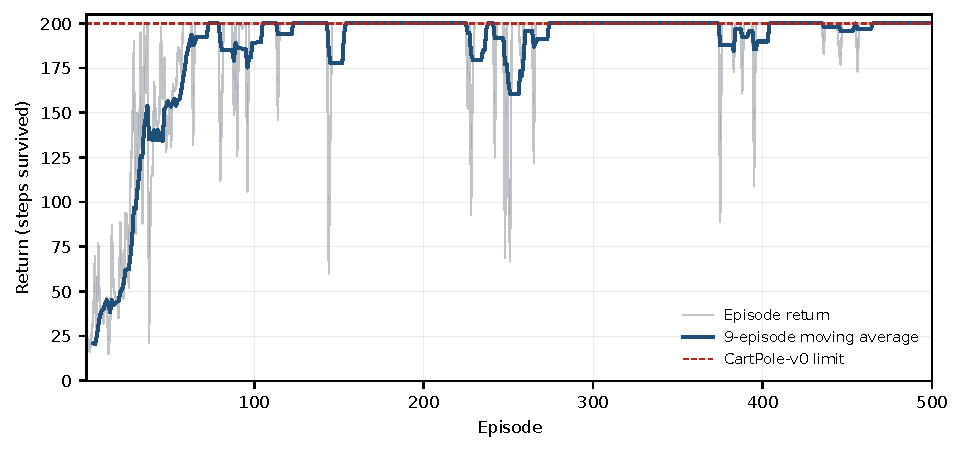
\includegraphics[width=\linewidth]{ppo_return.pdf}
  \caption{Episode returns and their nine-episode moving average. The dashed
  horizontal line marks the 200-step limit of CartPole-v0.}
  \label{fig:return}
\end{figure}

Figure~\ref{fig:return} shows the full measured sequence rather than only a
smoothed curve. The first 100 episodes average 140.26 returns. Control is
already nontrivial, but initial states and sampled actions still lead to
variable, shorter episodes. Growth continues through the early hundreds of
episodes as the actor assigns more mass to actions that preserve balance and
the critic improves the relative signal.

Over the final 100 episodes, the mean return is 199.19, the minimum is 173,
and 96 episodes meet the 200-step limit. The nine-episode average has small
local dips after some long high-return stretches. This behavior is consistent
with continued action sampling and randomized initial states: a policy with
strong average control can still take an unfavorable action or begin closer
to a failure boundary. The curve therefore supports consistently strong
control within the evaluation window, while retaining visible episode-level
variation.

\section{Limitations}\label{sec:limits}

The experiment evaluates one seed and one prescribed configuration. It does
not estimate variance across training runs or isolate the effect of changing
one hyperparameter. Episode returns are truncated at 200, so the reported
maximum is a lower bound on how long a successful policy could have continued.
Testing an environment without that time limit, or with a longer limit, would
be the direct test of long-horizon balancing. That additional experiment is
outside the short-assignment scope.

The implementation also follows the supplied environment wrapper, which
combines termination and truncation in the \texttt{done} flag. The final
transition therefore does not bootstrap from the post-limit state. This is a
documented feature of the starter training loop, not evidence that the policy
would be unable to continue.

\section{Conclusion}\label{sec:conclusion}

The implemented actor-critic update samples actions from a state-dependent
policy, turns TD errors into GAE advantages, and optimizes a clipped PPO
objective alongside a value-regression loss. The measured fixed-seed run
improves from a first-100 mean return of 140.26 to a final-100 mean of 199.19,
with 96 of the last 100 episodes reaching the environment's 200-step limit.
The result demonstrates effective finite-horizon control and is reported with
the limitations of truncation, single-seed evidence, and the documented
compatibility layer.

\begingroup
\small
\setlength{\bibsep}{2pt}
\bibliographystyle{plainnat}
\bibliography{reference}
\endgroup

\end{document}
